\documentclass{standalone}
\usepackage{tikz}
\usetikzlibrary{patterns, positioning}


\begin{document}
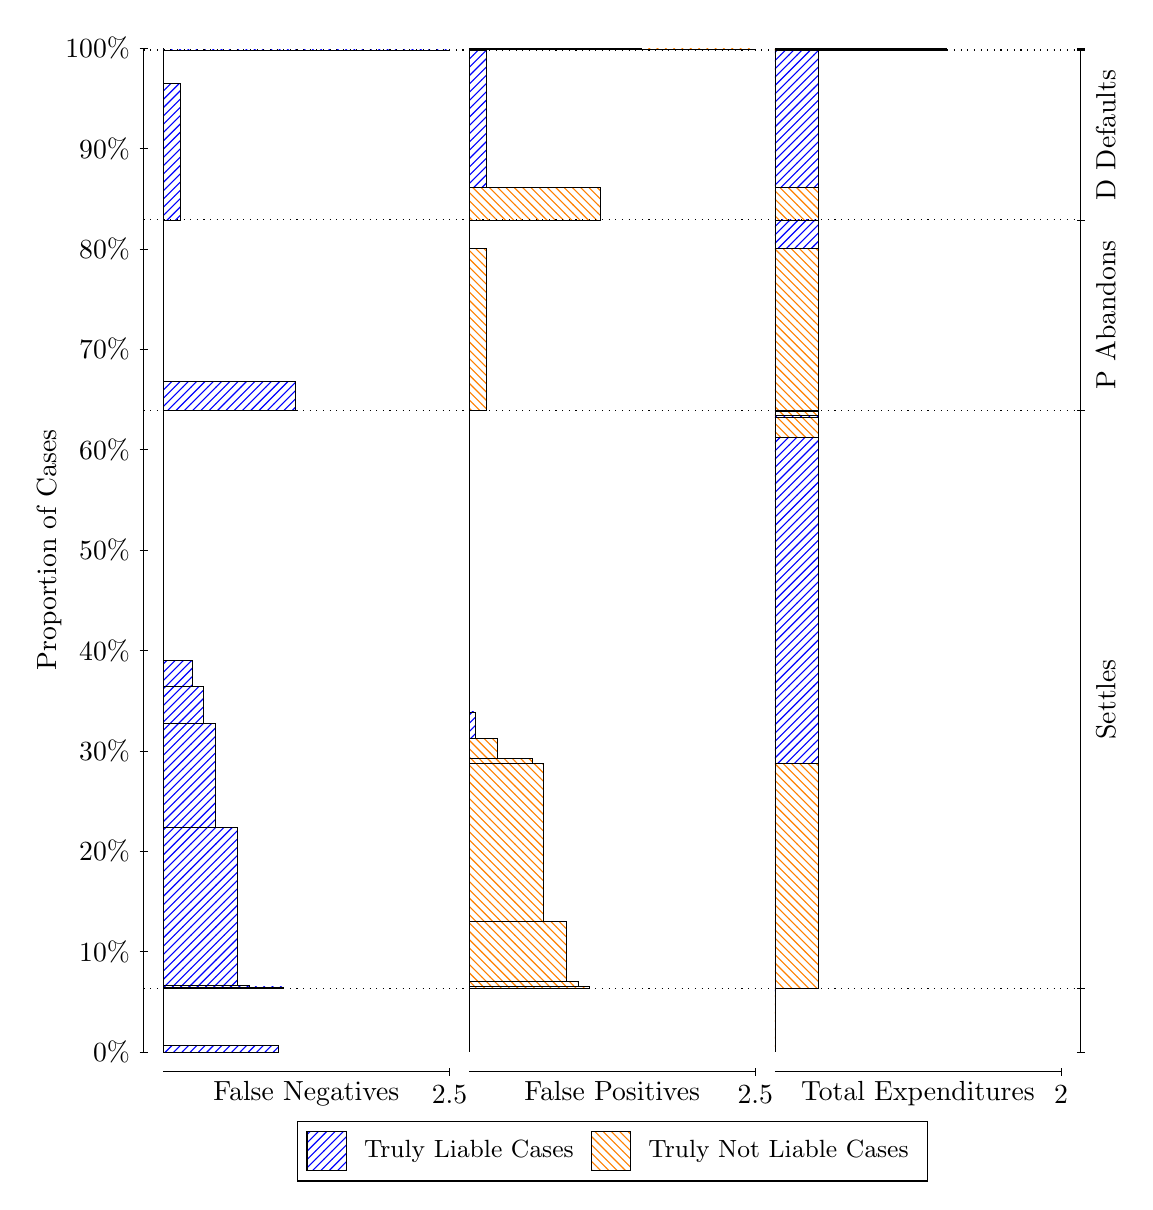
\begin{tikzpicture}
\draw[black, very thin] (1.5,1.75) -- (1.5,14.5);
\node[rotate=90, text=black, anchor=center] at (0.3, 8.125) {Proportion of Cases};
\draw[black, very thin] (1.45,1.75) -- (1.55,1.75);
\node[text=black, anchor=east] at (1.45, 1.75) {0\%};
\draw[black, very thin] (1.45,3.025) -- (1.55,3.025);
\node[text=black, anchor=east] at (1.45, 3.025) {10\%};
\draw[black, very thin] (1.45,4.3) -- (1.55,4.3);
\node[text=black, anchor=east] at (1.45, 4.3) {20\%};
\draw[black, very thin] (1.45,5.575) -- (1.55,5.575);
\node[text=black, anchor=east] at (1.45, 5.575) {30\%};
\draw[black, very thin] (1.45,6.85) -- (1.55,6.85);
\node[text=black, anchor=east] at (1.45, 6.85) {40\%};
\draw[black, very thin] (1.45,8.125) -- (1.55,8.125);
\node[text=black, anchor=east] at (1.45, 8.125) {50\%};
\draw[black, very thin] (1.45,9.4) -- (1.55,9.4);
\node[text=black, anchor=east] at (1.45, 9.4) {60\%};
\draw[black, very thin] (1.45,10.675) -- (1.55,10.675);
\node[text=black, anchor=east] at (1.45, 10.675) {70\%};
\draw[black, very thin] (1.45,11.95) -- (1.55,11.95);
\node[text=black, anchor=east] at (1.45, 11.95) {80\%};
\draw[black, very thin] (1.45,13.225) -- (1.55,13.225);
\node[text=black, anchor=east] at (1.45, 13.225) {90\%};
\draw[black, very thin] (1.45,14.5) -- (1.55,14.5);
\node[text=black, anchor=east] at (1.45, 14.5) {100\%};

\draw[black, very thin] (13.4,1.75) -- (13.4,14.5);
\draw[black, very thin] (13.35,1.75) -- (13.45,1.75);
\node[anchor=west] at (13.35, 1.75) {};
\draw[black, very thin] (13.35,2.5554) -- (13.45,2.5554);
\node[anchor=west] at (13.35, 2.5554) {};
\draw[black, very thin] (13.35,9.9018) -- (13.45,9.9018);
\node[anchor=west] at (13.35, 9.9018) {};
\draw[black, very thin] (13.35,12.318) -- (13.45,12.318);
\node[anchor=west] at (13.35, 12.318) {};
\draw[black, very thin] (13.35,14.471) -- (13.45,14.471);
\node[anchor=west] at (13.35, 14.471) {};
\draw[black, very thin] (13.35,14.483) -- (13.45,14.483);
\node[anchor=west] at (13.35, 14.483) {};
\draw[black, very thin] (13.35,14.5) -- (13.45,14.5);
\node[anchor=west] at (13.35, 14.5) {};

\draw[black, very thin, pattern color=blue, pattern=north east lines] (1.75,1.75) rectangle (3.2033,1.8347);
\draw[black, very thin, pattern color=orange, pattern=north west lines] (1.75,1.8347) rectangle (1.75,2.5554);
\draw[black, very thin, pattern color=blue, pattern=north east lines] (1.75,2.5554) rectangle (3.276,2.5771);
\draw[black, very thin, pattern color=blue, pattern=north east lines] (1.75,2.5771) rectangle (2.84,2.5912);
\draw[black, very thin, pattern color=blue, pattern=north east lines] (1.75,2.5912) rectangle (2.6947,4.5978);
\draw[black, very thin, pattern color=blue, pattern=north east lines] (1.75,4.5978) rectangle (2.404,5.9184);
\draw[black, very thin, pattern color=blue, pattern=north east lines] (1.75,5.9184) rectangle (2.2587,6.388);
\draw[black, very thin, pattern color=blue, pattern=north east lines] (1.75,6.388) rectangle (2.1133,6.7272);
\draw[black, very thin, pattern color=orange, pattern=north west lines] (1.75,6.7272) rectangle (1.75,9.9018);
\draw[black, very thin, pattern color=blue, pattern=north east lines] (1.75,9.9018) rectangle (3.4213,10.266);
\draw[black, very thin, pattern color=orange, pattern=north west lines] (1.75,10.266) rectangle (1.75,12.318);
\draw[black, very thin, pattern color=blue, pattern=north east lines] (1.75,12.318) rectangle (1.968,14.055);
\draw[black, very thin, pattern color=orange, pattern=north west lines] (1.75,14.055) rectangle (1.75,14.471);
\draw[black, very thin, pattern color=blue, pattern=north east lines] (1.75,14.471) rectangle (5.3833,14.476);
\draw[black, very thin, pattern color=orange, pattern=north west lines] (1.75,14.476) rectangle (1.75,14.483);
\draw[black, very thin, pattern color=orange, pattern=north west lines] (1.75,14.483) rectangle (1.75,14.488);
\draw[black, very thin, pattern color=blue, pattern=north east lines] (1.75,14.488) rectangle (1.75,14.5);
\draw[black, very thin, pattern color=orange, pattern=north west lines] (5.6333,1.75) rectangle (5.6333,2.4706);
\draw[black, very thin, pattern color=blue, pattern=north east lines] (5.6333,2.4706) rectangle (5.6333,2.5554);
\draw[black, very thin, pattern color=orange, pattern=north west lines] (5.6333,2.5554) rectangle (7.1593,2.5784);
\draw[black, very thin, pattern color=orange, pattern=north west lines] (5.6333,2.5784) rectangle (7.014,2.6477);
\draw[black, very thin, pattern color=orange, pattern=north west lines] (5.6333,2.6477) rectangle (6.8687,3.4112);
\draw[black, very thin, pattern color=orange, pattern=north west lines] (5.6333,3.4112) rectangle (6.578,5.4178);
\draw[black, very thin, pattern color=orange, pattern=north west lines] (5.6333,5.4178) rectangle (6.4327,5.4751);
\draw[black, very thin, pattern color=orange, pattern=north west lines] (5.6333,5.4751) rectangle (5.9967,5.7299);
\draw[black, very thin, pattern color=blue, pattern=north east lines] (5.6333,5.7299) rectangle (5.706,6.0692);
\draw[black, very thin, pattern color=blue, pattern=north east lines] (5.6333,6.0692) rectangle (5.6333,9.9018);
\draw[black, very thin, pattern color=orange, pattern=north west lines] (5.6333,9.9018) rectangle (5.8513,11.954);
\draw[black, very thin, pattern color=blue, pattern=north east lines] (5.6333,11.954) rectangle (5.6333,12.318);
\draw[black, very thin, pattern color=orange, pattern=north west lines] (5.6333,12.318) rectangle (7.3047,12.734);
\draw[black, very thin, pattern color=blue, pattern=north east lines] (5.6333,12.734) rectangle (5.8513,14.471);
\draw[black, very thin, pattern color=orange, pattern=north west lines] (5.6333,14.471) rectangle (5.6333,14.478);
\draw[black, very thin, pattern color=blue, pattern=north east lines] (5.6333,14.478) rectangle (5.6333,14.483);
\draw[black, very thin, pattern color=orange, pattern=north west lines] (5.6333,14.483) rectangle (9.2667,14.488);
\draw[black, very thin, pattern color=blue, pattern=north east lines] (5.6333,14.488) rectangle (7.8133,14.5);
\draw[black, very thin, pattern color=orange, pattern=north west lines] (9.5167,1.75) rectangle (9.5167,2.4706);
\draw[black, very thin, pattern color=blue, pattern=north east lines] (9.5167,2.4706) rectangle (9.5167,2.5554);
\draw[black, very thin, pattern color=orange, pattern=north west lines] (9.5167,2.5554) rectangle (10.062,5.4178);
\draw[black, very thin, pattern color=blue, pattern=north east lines] (9.5167,5.4178) rectangle (10.062,9.5539);
\draw[black, very thin, pattern color=orange, pattern=north west lines] (9.5167,9.5539) rectangle (10.062,9.8087);
\draw[black, very thin, pattern color=blue, pattern=north east lines] (9.5167,9.8087) rectangle (10.062,9.8303);
\draw[black, very thin, pattern color=orange, pattern=north west lines] (9.5167,9.8303) rectangle (10.062,9.8876);
\draw[black, very thin, pattern color=blue, pattern=north east lines] (9.5167,9.8876) rectangle (10.062,9.9018);
\draw[black, very thin, pattern color=orange, pattern=north west lines] (9.5167,9.9018) rectangle (10.062,11.954);
\draw[black, very thin, pattern color=blue, pattern=north east lines] (9.5167,11.954) rectangle (10.062,12.318);
\draw[black, very thin, pattern color=orange, pattern=north west lines] (9.5167,12.318) rectangle (10.062,12.734);
\draw[black, very thin, pattern color=blue, pattern=north east lines] (9.5167,12.734) rectangle (10.062,14.471);
\draw[black, very thin, pattern color=orange, pattern=north west lines] (9.5167,14.471) rectangle (11.697,14.478);
\draw[black, very thin, pattern color=blue, pattern=north east lines] (9.5167,14.478) rectangle (11.697,14.483);
\draw[black, very thin, pattern color=orange, pattern=north west lines] (9.5167,14.483) rectangle (11.697,14.488);
\draw[black, very thin, pattern color=blue, pattern=north east lines] (9.5167,14.488) rectangle (11.697,14.5);
\draw[black, dotted] (1.5,2.5554) -- (13.4,2.5554);
\draw[black, dotted] (1.5,9.9018) -- (13.4,9.9018);
\draw[black, dotted] (1.5,12.318) -- (13.4,12.318);
\draw[black, dotted] (1.5,14.471) -- (13.4,14.471);
\draw[black, dotted] (1.5,14.483) -- (13.4,14.483);
\draw[black, very thin] (1.75,1.5) -- (5.3833,1.5);
\node[text=black, anchor=north] at (3.5667, 1.5) {False Negatives};
\draw[black, very thin] (5.3833,1.45) -- (5.3833,1.55);
\node[text=black, anchor=north] at (5.3833, 1.45) {2.5};

\draw[black, very thin] (5.6333,1.5) -- (9.2667,1.5);
\node[text=black, anchor=north] at (7.45, 1.5) {False Positives};
\draw[black, very thin] (9.2667,1.45) -- (9.2667,1.55);
\node[text=black, anchor=north] at (9.2667, 1.45) {2.5};

\draw[black, very thin] (9.5167,1.5) -- (13.15,1.5);
\node[text=black, anchor=north] at (11.333, 1.5) {Total Expenditures};
\draw[black, very thin] (13.15,1.45) -- (13.15,1.55);
\node[text=black, anchor=north] at (13.15, 1.45) {2};


\node[text=black, centered, rotate=90] at (13.72, 6.2286) {Settles};
\node[text=black, centered, rotate=90] at (13.72, 11.11) {P Abandons};
\node[text=black, centered, rotate=90] at (13.72, 13.395) {D Defaults};



\draw (7.449999999999999,1.5) node[draw=none] (baseCoordinate) {};
\begin{scope}[align=center]
        \matrix[scale=0.5, draw=black, below=0.5cm of baseCoordinate, nodes={draw}, column sep=0.1cm]{
            \node[rectangle, draw, minimum width=0.5cm, minimum height=0.5cm, pattern color=blue, pattern=north east lines] {}; &
            \node[draw=none, font=\small, text=black] (B) {Truly Liable Cases}; &
            \node[rectangle, draw, minimum width=0.5cm, minimum height=0.5cm, pattern color=orange, pattern=north west lines] {}; &
            \node[draw=none, font=\small, text=black] (B) {Truly Not Liable Cases}; \\
            };
\end{scope}

\end{tikzpicture}
\end{document}